\documentclass{mcmthesis}
\usepackage{indentfirst}
\setlength{\parindent}{2em}
\mcmsetup{CTeX = true,   % 使用 CTeX 套装时,设置为 true
        tcn = 0000, problem = C,% 队伍控制号码,接受一个字符串作为值;选题,接受一个字符串作为值;
        sheet = true, %为真时将输出摘要页,否则不输出;默认为 true。
        color = red,  %设置控制页的题目号的颜色
        titleinsheet = true, %为真时将在摘要页输出标题,否则不输出;默认为 false。
        keywordsinsheet = true,%为真时将在摘要页输出关键字,否则不输出;默认为 false。
        titlepage = false,%为真时将输出标题页,否则不输出;默认为 true。
        abstract = true}%为真时将在标题页输出摘要和关键词,否则不输出;默认值为 true。
\usepackage{palatino}  %控制正文字体,若是不喜欢可以注释掉。
\usepackage{lipsum}
\title{The \LaTeX{} Template for MCM Version \MCMversion}
\author{\url{http://www.latexstudio.net}\\[3pt]  \href{http://www.latexstudio.net/}
  {
\includegraphics[width=7cm]{mcmthesis-logo}}}
\date{\today}

\makeatletter
\renewcommand*\l@section{\@dottedtocline{1}{12pt}{12pt}}
\makeatother

\begin{document}
\begin{abstract}
	The Abstract should be
	structured to include the following details: Background,
	the context and purpose of the study; Results, the main
	findings; Conclusions, brief summary and potential im-
	plications. Please minimize the use of abbreviations and
	do not cite references in the abstract.
	\begin{keywords}
		keyword1; keyword2
	\end{keywords}
\end{abstract}

\maketitle

\tableofcontents
\newpage

\section{Introduction}
	\subsection{Problem Background}
		\par As narcotic analgesics, opioids are primarily used for pain relief and anesthesia to reduce patients' suffering, which contribute a lot to modern medicine since its appearance. However, it also has many side effects, including itchiness, nausea, respiratory depression, constipation, and, what counts most, addiction. Considering the adverse effects above, we tend to enforce the regulation of opioids to reduce the risk of addiction.
		
		Nowadays, The United States is undergoing one of its worst drug crises caused by opioids. Hundreds of people die from opioid-related overdoses while more and more Americans are suffering from opioid addiction. The crisis has reached such a scale that, beyond the risks it brings to public health, the loss of people with advanced degrees will curb the development of economy and national security.
		
		With the data offered by Drug Enforcement Administration's Office of Diversion Control about the situation of drug abusing in five states, we can know more about the characteristics of opioid epidemic and find out the factors contributing to the growth in opioid use and addiction, so that we can set a therapy to alleviate the problem.


	\subsection{View of Our Work}

		\par For the first Problem, we build a LSTM(Long Short Term Memory)Neural Network Modle to predict the trendency of drug abusing.This model can take the time sequence of pentential drug abuse cases in countise  as input. The output will be the predict time sequence of pentential drug abuse cases in the future. 
		\par By comparing the prediction for the feture and last year's data, we can clearly find which place in all countis has the tendency to increase and view these counties as the result to be specific concerned. We found that the drug abuse tend to be increase in the counties which is historically have problem with drug abuse.
		
		\par For the second problem, we need to take the cencus data into consideration. So we make a new input branch for our model to obtain the inflence of social-economy influence. The new branch consists of three autoencode layers, the output of the autoendoer can capture the most salient features of the training data. 
		\par And then we caculate the correlation coefficient matrix for all the input and output data.So that princple variables will be find to be the >>>> following the change of vari >>>>> we get we find  >>>> contributes most to the opion crsis.
		
		\par Finally, we caculate different the future results under different pramemters.And get the best range for the pramemters to be controled in.
	\subsection{Assumptions}

		\par Due to the limited data of the pentential drug abuse cases, and other soc........,we use the 
		following assumptions to complete our model. These simplified assumptions will be used through our paper and can be improved with more reliable data:
		\begin{itemize}
			\item The count of drug abuse cases in a county can be regared as a presentation of the total drug abuse cases in this county.
			\item The total drug abuse cases in a county is proportional to the count data we get. This is reasonable because ..................
			\item Neglect the diffierence of opioid medicine on kind, we view all the instance of opioid as one to our model.  
		\end{itemize}
\begin{tabular}{cp{0.6\textwidth}} 
	\toprule
	 Symbols & Description\\
	\midrule
	 $x$ & position \\
	 $v$ & velocity \\
	 $a$ & acceleration \\
	 $t$ & time \\
	 $F$ & force\\
	\bottomrule
\end{tabular}


\section{Model One - A Pretrained Neural Network}
	\par In the first part of the problem one, we pretrain the weight of a neural and a new kind of way to train the weight of a neural network to describe the spread and characteristics of the reported synthetic opioid and heroin incidents in and between the five states. 
	\subsection{Assumptions}
		\begin{itemize}
			\item We view the spread of the cases as a mulity variables time sequence. And there are $461$ counties which have drug abuse cases in these five states,so the spread of drug abuse cases in $t$ year is viewed as a time sequence like this: 
				$$X(t) = ( x_{1}(t), x_{2}(t), ..., x_{461}(t) )$$
				and for the next,  $t+1$ year should be like this:
				$$X(t) = ( x_{1}(t+1), x_{2}(t+1), ..., x_{461}(t+1) )$$
			\item The spread of opiod crisis has relationship with the location information of counties.Because the spread of opiod crisis is clearly with respece to the space spread.
			\item The potential drug abuse cases in a county can be measured by the drug identification counts. To be simple, we assume the potential cases is proportional to the identification counts. 
		\end{itemize}
	\subsection{Establishing the model}
	\par In each year, the time sequence $X(t)$ is with respect to the last year's $X(t-1)$, we can use a variable $w_{i, j}$ to describe the influence from last year's $x_{j}$ to the next year's $x_{i}$,
	we can write them in the form of matrixs:
		$$ X(t-1)W = X(t) $$
	its topological graph will be like the following Figure \ref{fig:Topological Graph of Model One}:
		\begin{figure}[h]
			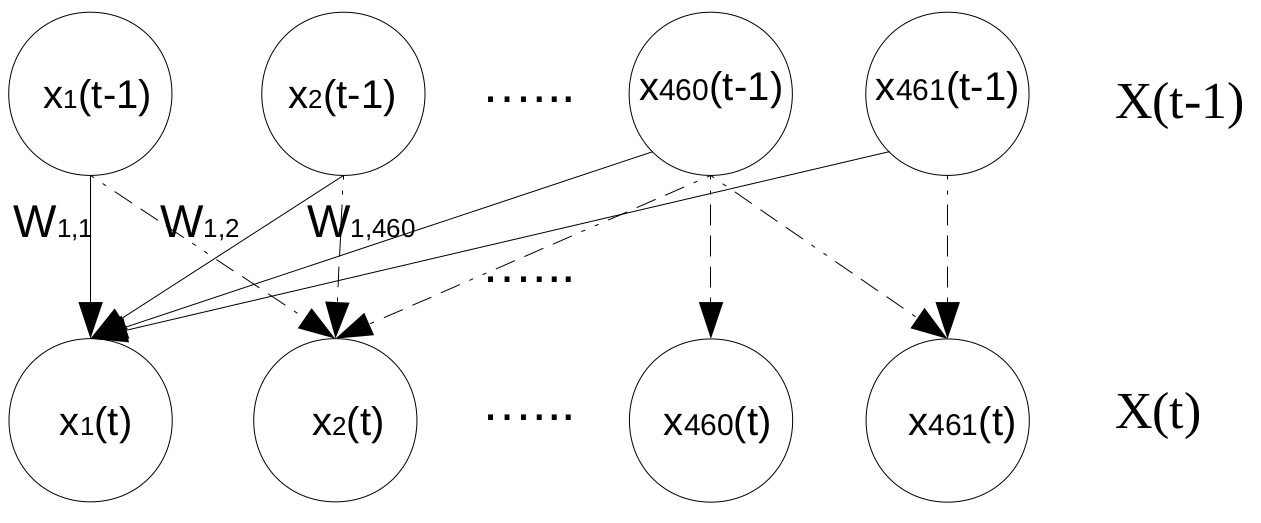
\includegraphics[width=12cm]{01_Model_One_diagram.png}
			\centering
			\caption{Model One Topological Graph} \label{fig:Topological Graph of Model One}
		\end{figure}
	\par According to our assumption, there is negative correlation between the value $w_{i, j}$ and the distance spreated from each other for two county.The influence of one county that described with $W_{:, j}$ will drop quickly with the distance increasing. Gauss Function is used to describe the spreaded influence as Figure \ref{fig:Gauss Weight Function}:
		\begin{figure}
			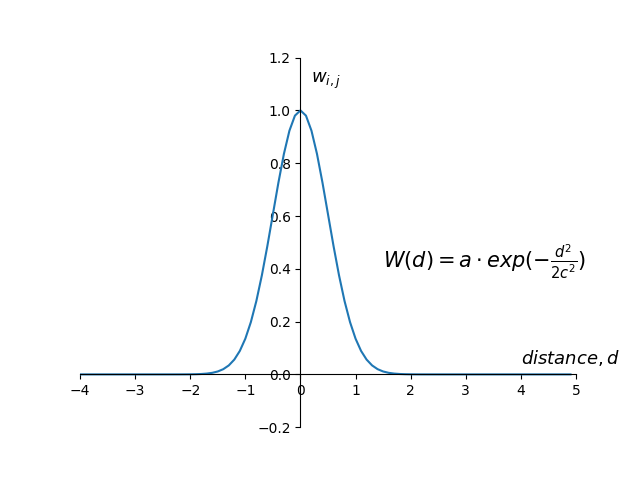
\includegraphics[width=12cm]{02_W_Gauss_Func.png}
			\centering
			\caption{Gauss Weight Function} \label{fig:Gauss Weight Function}
		\end{figure}
	\par We use this Function \ref{func:Gauss Weight Function} to fit the $W$'s value:
		
		$$W(d)= a \cdot exp(-\frac{d^2}{2c^2}) \label{func:Gauss Weight Function}$$

	\par In this function, the pramemter $a_{i, j}$ can control the capbility of last year's counties to contribute to the next year's counties's pontential drug cases. The pramemter $c_{i, j}$ can control the influence radius.
	\par A \textbf{Spcefic Designed Back-Propagation Algorithm} is used to modify the two parameters step by step. 
	\par To caculate the appropriate values for the $a_{i, j}$ and $c_{i, j}$, we regard the $w_{i, j}$ as the weights of a neural network with only a dense layer and define a loss Function \ref{func:Loss function for model one} to make our parameter more reasonable.
		$$f_{loss}(W) = (\hat{X(t)} - X(t))^2 \label{func:Loss function for model one} $$
	\par Here, the $\hat{X(t)}$ is the prediction of drug abuse sperad, the function can also be written as:
		$$ f_{loss}(W) = X(t-1) \cdot W_{i, j} - X(t))^2 $$
	\par According to the chain rule of calculus, we can compute the derivatives of functions formed by composing other functions whose derivatives are known. So we can compute the derivatives of the $f_{loss}$ about $c_{i, j}$ like this:
		$$
		\frac{\partial f_{loss}}{\partial c_{i,j}} = \frac{\partial f_{loss}}{\partial x_{i,j}}
		\frac{\partial x_{i, j}}{\partial w_{i,j}} \frac{\partial w_{i,j}}{\partial c_{i, j}}
		$$
	\par Similarly, we can get the derivatives about $a$:
		$$
		\frac{\partial f_{loss}}{\partial c_{i,j}} = \frac{\partial f_{loss}}{\partial x_{i,j}}
		\frac{\partial x_{i, j}}{\partial w_{i,j}} \frac{\partial w_{i,j}}{\partial a_{i, j}}
		$$
	\subsection{Results and Improvement of Model One}
	
	\par Then we can use this function to train the $C = c_{i, j}$ and $A = a_{i, j}$ to a appropriate value. The parameter $C$ represent the county's influence radius, and the praameter $c$ represent the county's ability to influence other counties around. We can get the figure 
	
	% 缺一张图!!!!!!!!!!!!!!!!!!!!!!!!!!!!!!!!!!!!!!!!!!!!!
	\par picture!!!!!!!!!!!!!!!!!!!!!!!!!!!!!!!!!!!!!!!!!!!!!!!!!!!!!!!!!
	\par picture!!!!!!!!!!!!!!!!!!!!!!!!!!!!!!!!!!!!!!!!!!!!!!!!!!!!!!!!!
	\par picture!!!!!!!!!!!!!!!!!!!!!!!!!!!!!!!!!!!!!!!!!!!!!!!!!!!!!!!!!
	\par picture!!!!!!!!!!!!!!!!!!!!!!!!!!!!!!!!!!!!!!!!!!!!!!!!!!!!!!!!!
	\par picture!!!!!!!!!!!!!!!!!!!!!!!!!!!!!!!!!!!!!!!!!!!!!!!!!!!!!!!!!
	\par picture!!!!!!!!!!!!!!!!!!!!!!!!!!!!!!!!!!!!!!!!!!!!!!!!!!!!!!!!!
	\par picture!!!!!!!!!!!!!!!!!!!!!!!!!!!!!!!!!!!!!!!!!!!!!!!!!!!!!!!!!
	\par picture!!!!!!!!!!!!!!!!!!!!!!!!!!!!!!!!!!!!!!!!!!!!!!!!!!!!!!!!!
	\par picture!!!!!!!!!!!!!!!!!!!!!!!!!!!!!!!!!!!!!!!!!!!!!!!!!!!!!!!!!
	\par picture!!!!!!!!!!!!!!!!!!!!!!!!!!!!!!!!!!!!!!!!!!!!!!!!!!!!!!!!!

	\par In this figure, it shows the spread of the opioid crisis.Every county in this diagram has a circle filled in different color. The $C$ is represented by the radius sizes of circles which means how long a county can spread or releave the crisis to others. The $A$ is represented by the color of the circle which shows the ability of the county to spread crisis to others.
	\par Till now we can use the model to describe the spread of opioid crisis
	but we can't identify possible locations where specific opioid use might have started. So we are going to reversal our model to trace back the possible locations. 
	% -------------------------------------------------------------------------------------------
	
	\par We want to make the reverse our model to trace back to the sources in each five states.
	So our model will be 
	\par With these 
	
	
	
	%---------------------------------------------------------------------------------------------
	\par With the reversed model we can date back to the start of specific opioid use,which is shown in the picture below, these countise in each five sates are the possible locations we assert.
	\par false picture !!!!!!!!!!!!!!!!!!!!!!!!!!!!!!!!!!!!!!!!!!!!!!!!!
	\par false picture !!!!!!!!!!!!!!!!!!!!!!!!!!!!!!!!!!!!!!!!!!!!!!!!!
	\par false picture !!!!!!!!!!!!!!!!!!!!!!!!!!!!!!!!!!!!!!!!!!!!!!!!!
	\par false picture !!!!!!!!!!!!!!!!!!!!!!!!!!!!!!!!!!!!!!!!!!!!!!!!!
	\par false picture !!!!!!!!!!!!!!!!!!!!!!!!!!!!!!!!!!!!!!!!!!!!!!!!!
	\par false picture !!!!!!!!!!!!!!!!!!!!!!!!!!!!!!!!!!!!!!!!!!!!!!!!!
	\par false picture !!!!!!!!!!!!!!!!!!!!!!!!!!!!!!!!!!!!!!!!!!!!!!!!!
	
	\par In this section, we create a specfic neural network, and use specific designed Back-Propagation Algorithm to get two parameters which can describe the spread of the opioid crisis. But the disadvantange of the model is that it only take the $X(t-1)$ in to consideration, and simply trow away all the data before,such as $X(t-2), X(t-3),X(t-4)...$. This can cause inaccuracy when it pridict a long term future.
	
	
\section{Model Two: A LSTM Neural Network}
	

\[
  \begin{pmatrix}{*{20}c}
  {a_{11} } & {a_{12} } & {a_{13} }  \\
  {a_{21} } & {a_{22} } & {a_{23} }  \\
  {a_{31} } & {a_{32} } & {a_{33} }  \\
  \end{pmatrix}
  = \frac{{Opposite}}{{Hypotenuse}}\cos ^{ - 1} \theta \arcsin \theta
\]
\lipsum[9]

\[
  p_{j}=\begin{cases} 0,&\text{if $j$ is odd}\\
  r!\,(-1)^{j/2},&\text{if $j$ is even}
  \end{cases}
\]

\lipsum[10]

\[
  \arcsin \theta  =
  \mathop{{\int\!\!\!\!\!\int\!\!\!\!\!\int}\mkern-31.2mu
  \bigodot}\limits_\varphi
  {\mathop {\lim }\limits_{x \to \infty } \frac{{n!}}{{r!\left( {n - r}
  \right)!}}} \eqno (1)
\]

\section{Calculating and Simplifying the Model  }
\lipsum[11]

\section{The Model Results}
\lipsum[6]

\section{Validating the Model}
\lipsum[9]

\section{Conclusions}
\lipsum[6]

\section{A Summary}
\lipsum[6]

\section{Evaluate of the Mode}

\section{Strengths and weaknesses}
\lipsum[12]

\subsection{Strengths}
\begin{itemize}
\item \textbf{Applies widely}\\
This  system can be used for many types of airplanes, and it also
solves the interference during  the procedure of the boarding
airplane,as described above we can get to the  optimization
boarding time.We also know that all the service is automate.
\item \textbf{Improve the quality of the airport service}\\
Balancing the cost of the cost and the benefit, it will bring in
more convenient  for airport and passengers.It also saves many
human resources for the airline. \item \textbf{}
\end{itemize}

\begin{thebibliography}{99}
\bibitem{1} D.~E. KNUTH   The \TeX{}book  the American
Mathematical Society and Addison-Wesley
Publishing Company , 1984-1986.
\bibitem{2}Lamport, Leslie,  \LaTeX{}: `` A Document Preparation System '',
Addison-Wesley Publishing Company, 1986.
\bibitem{3}\url{http://www.latexstudio.net/}
\bibitem{4}\url{http://www.chinatex.org/}
\end{thebibliography}

\begin{appendices}

\section{First appendix}

\lipsum[13]

Here are simulation programmes we used in our model as follow.\\

\textbf{\textcolor[rgb]{0.98,0.00,0.00}{Input matlab source:}}
\lstinputlisting[language=Matlab]{./code/mcmthesis-matlab1.m}

\section{Second appendix}

some more text \textcolor[rgb]{0.98,0.00,0.00}{\textbf{Input C++ source:}}
\lstinputlisting[language=C++]{./code/mcmthesis-sudoku.cpp}

\end{appendices}
\end{document}

%%
%% This work consists of these files mcmthesis.dtx,
%%                                   figures/ and
%%                                   code/,
%% and the derived files             mcmthesis.cls,
%%                                   mcmthesis-demo.tex,
%%                                   README,
%%                                   LICENSE,
%%                                   mcmthesis.pdf and
%%                                   mcmthesis-demo.pdf.
%%
%% End of file `mcmthesis-demo.tex'.